\documentclass[11pt,oneside]{article}
\usepackage[T1]{fontenc}
\usepackage[utf8]{inputenc}
% \usepackage{lmodern}
%\usepackage[adobe-utopia,uppercase=upright,greeklowercase=upright]{mathdesign}
\usepackage[adobe-utopia]{mathdesign}
%\usepackage{minionpro}
% \usepackage{pifont}
% \usepackage{amssymb}
\usepackage{amsmath}
\usepackage[francais]{babel}
% \usepackage[francais]{varioref}
\usepackage[dvips]{graphicx}

\usepackage{framed}
\usepackage[normalem]{ulem}
\usepackage{fancyhdr}
\usepackage{titlesec}
\usepackage{vmargin}
\usepackage{longtable}

\usepackage{ifthen}


%\usepackage{epsfig}
\usepackage{subfig}

\usepackage{multirow}
\usepackage{multicol} % Portions de texte en colonnes
\usepackage{flafter}%floatants après la référence



\usepackage{color}
\usepackage{colortbl}


\definecolor{gris25}{gray}{0.75}
\definecolor{bleu}{RGB}{18,33,98}
\definecolor{bleuf}{RGB}{42,94,171}
\definecolor{bleuc}{RGB}{231,239,247}
\definecolor{rougef}{RGB}{185,18,27}
\definecolor{rougec}{RGB}{255,230,231}
\definecolor{vertf}{RGB}{103,126,82}
\definecolor{vertc}{RGB}{220,255,191}

\newenvironment{rem}[1][\hsize]%
{%
    \def\FrameCommand
    {%
\rotatebox{90}{\textit{\textsf{Remarque}}} 
        {\color{bleuf}\vrule width 3pt}%
        \hspace{0pt}%must no space.
        \fboxsep=\FrameSep\colorbox{bleuc}%
    }%
    \MakeFramed{\hsize#1\advance\hsize-\width\FrameRestore}%
}%
{\endMakeFramed}%


\newenvironment{savoir}[1][\hsize]%
{%
    \def\FrameCommand
    {%
\rotatebox{90}{\textit{\textsf{Savoir}}} 
        {\color{bleuf}\vrule width 3pt}%
        \hspace{0pt}%must no space.
        \fboxsep=\FrameSep\colorbox{bleuc}%
    }%
    \MakeFramed{\hsize#1\advance\hsize-\width\FrameRestore}%
}%
{\endMakeFramed}%

\newenvironment{prob}[1][\hsize]%
{%
    \def\FrameCommand%
    {%
\rotatebox{90}{\textit{\textsf{ Problématique}}} 
        {\color{rougef}\vrule width 3pt}%
        \hspace{0pt}%must no space.
        \fboxsep=\FrameSep\colorbox{rougec}%
    }%
    \MakeFramed{\hsize#1\advance\hsize-\width\FrameRestore}%
}%
{\endMakeFramed}%

\newenvironment{obj}[1][\hsize]%
{%
    \def\FrameCommand%
    {%
\rotatebox{90}{\textit{\textsf{ $\;$}}} 
        {\color{rougef}\vrule width 3pt}%
        \hspace{0pt}%must no space.
        \fboxsep=\FrameSep\colorbox{rougec}%
    }%
    \MakeFramed{\hsize#1\advance\hsize-\width\FrameRestore}%
}%
{\endMakeFramed}%

\newenvironment{defi}[1][\hsize]%
{%
    \def\FrameCommand%
    {%
\rotatebox{90}{\textit{\textsf{Définition\\}}} 
        {\color{bleuf}\vrule width 3pt}%
        \hspace{0pt}%must no space.
        \fboxsep=\FrameSep\colorbox{bleuc}%
    }%
    \MakeFramed{\hsize#1\advance\hsize-\width\FrameRestore}%
}%
{\endMakeFramed}%


\newenvironment{hypo}[1][\hsize]%
{%
    \def\FrameCommand%
    {%
\rotatebox{90}{\textit{\textsf{Hypothèse\\}}} 
        {\color{bleuf}\vrule width 3pt}%
        \hspace{0pt}%must no space.
        \fboxsep=\FrameSep\colorbox{bleuc}%
    }%
    \MakeFramed{\hsize#1\advance\hsize-\width\FrameRestore}%
}%
{\endMakeFramed}%


\newenvironment{prop}[1][\hsize]%
{%
    \def\FrameCommand%
    {%
\rotatebox{90}{\textit{\textsf{Propriété\\}}} 
        {\color{bleuf}\vrule width 3pt}%
        \hspace{0pt}%must no space.
        \fboxsep=\FrameSep\colorbox{bleuc}%
    }%
    \MakeFramed{\hsize#1\advance\hsize-\width\FrameRestore}%
}%
{\endMakeFramed}%

\newenvironment{props}[1][\hsize]%
{%
    \def\FrameCommand%
    {%
\rotatebox{90}{\textit{\textsf{Propriétés\\}}} 
        {\color{bleuf}\vrule width 3pt}%
        \hspace{0pt}%must no space.
        \fboxsep=\FrameSep\colorbox{bleuc}%
    }%
    \MakeFramed{\hsize#1\advance\hsize-\width\FrameRestore}%
}%
{\endMakeFramed}%

\newenvironment{exemple}[1][\hsize]%
{%
    \def\FrameCommand%
    {%
\rotatebox{90}{\textit{\textsf{Exemple\\}}} 
        {\color{vertf}\vrule width 3pt}%
        \hspace{0pt}%must no space.
        \fboxsep=\FrameSep\colorbox{vertc}%
    }%
    \MakeFramed{\hsize#1\advance\hsize-\width\FrameRestore}%
}%
{\endMakeFramed}%

\newenvironment{resultat}[1][\hsize]%
{%
    \def\FrameCommand%
    {%
\rotatebox{90}{\textit{\textsf{Résultat\\}}} 
        {\color{rougef}\vrule width 3pt}%
        \hspace{0pt}%must no space.
        \fboxsep=\FrameSep\colorbox{rougec}%
    }%
    \MakeFramed{\hsize#1\advance\hsize-\width\FrameRestore}%
}%
{\endMakeFramed}%

\newenvironment{methode}[1][\hsize]%
{%
    \def\FrameCommand%
    {%
\rotatebox{90}{\textit{\textsf{Méthode\\}}} 
        {\color{rougef}\vrule width 3pt}%
        \hspace{0pt}%must no space.
        \fboxsep=\FrameSep\colorbox{rougec}%
    }%
    \MakeFramed{\hsize#1\advance\hsize-\width\FrameRestore}%
}%
{\endMakeFramed}%

\newenvironment{theo}[1][\hsize]%
{%
    \def\FrameCommand%
    {%
\rotatebox{90}{\textit{\textsf{Théorème\\}}} 
        {\color{rougef}\vrule width 3pt}%
        \hspace{0pt}%must no space.
        \fboxsep=\FrameSep\colorbox{rougec}%
    }%
    \MakeFramed{\hsize#1\advance\hsize-\width\FrameRestore}%
}%
{\endMakeFramed}%

\newenvironment{warn}[1][\hsize]%
{%
    \def\FrameCommand%
    {%
\rotatebox{90}{\textit{\textsf{Attention\\}}} 
        {\color{rougef}\vrule width 3pt}%
        \hspace{0pt}%must no space.
        \fboxsep=\FrameSep\colorbox{rougec}%
    }%
    \MakeFramed{\hsize#1\advance\hsize-\width\FrameRestore}%
}%
{\endMakeFramed}%

% \usepackage{pstricks}
%\usepackage{minitoc}
% \setcounter{minitocdepth}{4}

\setcounter{tocdepth}{2}

% \mtcselectlanguage{french} 

%\usepackage{draftcopy}% "Brouillon"
% \usepackage{floatflt}
\usepackage{psfrag}
%\usepackage{listings} % Permet d'insérer du code de programmation
\renewcommand{\baselinestretch}{1.2}

% Changer la numérotation des figures :
% ------------------------------------
% \makeatletter
% \renewcommand{\thefigure}{\ifnum \c@section>\z@ \thesection.\fi
%  \@arabic\c@figure}
% \@addtoreset{figure}{section}
% \makeatother
 


%%%%%%%%%%%%
% Définition des vecteurs %
%%%%%%%%%%%%
 \newcommand{\vect}[1]{\overrightarrow{#1}}

%%%%%%%%%%%%
% Définition des torseusr %
%%%%%%%%%%%%

 \newcommand{\torseur}[1]{%
\left\{{#1}\right\}
}

\newcommand{\torseurcin}[3]{%
\left\{\mathcal{#1} \left(#2/#3 \right) \right\}
}

\newcommand{\torseurstat}[3]{%
\left\{\mathcal{#1} \left(#2\rightarrow #3 \right) \right\}
}

 \newcommand{\torseurc}[8]{%
%\left\{#1 \right\}=
\left\{
{#1}
\right\}
 = 
\left\{%
\begin{array}{cc}%
{#2} & {#5}\\%
{#3} & {#6}\\%
{#4} & {#7}\\%
\end{array}%
\right\}_{#8}%
}

 \newcommand{\torseurcol}[7]{
\left\{%
\begin{array}{cc}%
{#1} & {#4}\\%
{#2} & {#5}\\%
{#3} & {#6}\\%
\end{array}%
\right\}_{#7}%
}

 \newcommand{\torseurl}[3]{%
%\left\{\mathcal{#1}\right\}_{#2}=%
\left\{%
\begin{array}{l}%
{#1} \\%
{#2} %
\end{array}%
\right\}_{#3}%
}

 \newcommand{\vectv}[3]{%
\vect{V\left( {#1} \in {#2}/{#3}\right)}
}


\newcommand{\vectf}[2]{%
\vect{R\left( {#1} \rightarrow {#2}\right)}
}

\newcommand{\vectm}[3]{%
\vect{\mathcal{M}\left( {#1}, {#2} \rightarrow {#3}\right)}
}


 \newcommand{\vectg}[3]{%
\vect{\Gamma \left( {#1} \in {#2}/{#3}\right)}
}

 \newcommand{\vecto}[2]{%
\vect{\Omega\left( {#1}/{#2}\right)}
}
% }$$\left\{\mathcal{#1} \right\}_{#2} =%
% \left\{%
% \begin{array}{c}%
%  #3 \\%
%  #4 %
% \end{array}%
% \right\}_{#5}}

%  ------------------------------------------
% | Modification du formatage des sections : | 
%  ------------------------------------------

% Grands titres :
% ---------------

\newcommand{\titre}[1]{%
\begin{center}
      \bigskip
      \rule{\textwidth}{1pt}
      \par\vspace{0.1cm}
      
      \textbf{\large #1}
      \par\rule{\textwidth}{1pt}
    \end{center}
    \bigskip
  }

% Supprime le numéro du chapitre dans la numérotation des sections:
% -----------------------------------------------------------------
\makeatletter
\renewcommand{\thesection}{\@arabic\c@section}
\makeatother


% \titleformat{\chapter}[display]
% {\normalfont\Large\filcenter}
% {}
% {1pc}
% {\titlerule[1pt]
%   \vspace{1pc}%
%   \Huge}[\vspace{1ex}%
% \titlerule]


%%%% Chapitres Comme PY Pechard %%%%%%%%%
% numéro du chapitre
\DeclareFixedFont{\chapnumfont}{OT1}{phv}{b}{n}{80pt}
% pour le mot « Chapitre »
\DeclareFixedFont{\chapchapfont}{OT1}{phv}{m}{it}{40pt}
% pour le titre
\DeclareFixedFont{\chaptitfont}{T1}{phv}{b}{n}{25pt}

\definecolor{gris}{gray}{0.75}
\titleformat{\chapter}[display]%
	{\sffamily}%
	{\filleft\chapchapfont\color{gris}\chaptertitlename\
	\\
	\vspace{12pt}
	\chapnumfont\thechapter}%
	{16pt}%
	{\filleft\chaptitfont}%
	[\vspace{6pt}\titlerule\titlerule\titlerule]

%%%%  Fin Chapitres Comme PY Pechard %%%%%%%%%


% Section, subsection, subsubsection sans serifs :
% % ----------------------------------------------

% \makeatletter
% \renewcommand{\section}{\@startsection{section}{0}{0mm}%
% {\baselineskip}{.3\baselineskip}%
% {\normalfont\sffamily\Large\textbf}}%
% \makeatother

\makeatletter
\renewcommand{\@seccntformat}[1]{{\textcolor{bleu}{\csname
the#1\endcsname}\hspace{0.5em}}}
\makeatother

\makeatletter
\renewcommand{\section}{\@startsection{section}{1}{\z@}%
                       {-4ex \@plus -1ex \@minus -.4ex}%
                       {1ex \@plus.2ex }%
                       {\normalfont\Large\sffamily\bfseries}}%
\makeatother
 
\makeatletter
\renewcommand{\subsection}{\@startsection {subsection}{2}{\z@}
                          {-3ex \@plus -0.1ex \@minus -.4ex}%
                          {0.5ex \@plus.2ex }%
                          {\normalfont\large\sffamily\bfseries}}
\makeatother
 
\makeatletter
\renewcommand{\subsubsection}{\@startsection {subsubsection}{3}{\z@}
                          {-2ex \@plus -0.1ex \@minus -.2ex}%
                          {0.2ex \@plus.2ex }%
                          {\normalfont\large\sffamily\bfseries}}
\makeatother
 
\makeatletter             
\renewcommand{\paragraph}{\@startsection{paragraph}{4}{\z@}%
                                    {-2ex \@plus-.2ex \@minus .2ex}%
                                    {0.1ex}%               
{\normalfont\sffamily\bfseries}}
\makeatother
 
\makeatletter
\renewcommand{\subparagraph}{\@startsection{subparagraph}{5}{\z@}%
                                       {-2ex \@plus-.1ex \@minus .2ex}%
                                       {0.1ex}%
				    {\normalfont\normalsize\sffamily\bfseries}}
\makeatletter
% \makeatletter
% \renewcommand{\subsection}{\@startsection{subsection}{1}{2mm}%
% {\baselineskip}{.3\baselineskip}%
% {\normalfont\sffamily\large\textbf}}%
% \makeatother
% 
% \makeatletter
% \renewcommand{\subsubsection}{\@startsection{subsubsection}{2}{4mm}%
% {\baselineskip}{.15\baselineskip}%
% {\normalfont\sffamily\large\textbf}}%
% \makeatother
% 
% \makeatletter
% \renewcommand{\paragraph}{\@startsection{paragraph}{3}{6mm}%
% {\baselineskip}{.15\baselineskip}%
% {\normalfont\sffamily\large\textbf}}%
% \makeatother
 
\setcounter{secnumdepth}{4}


%  --------
% | Marges |
%  --------


% \setmarginsrb{2.5cm}{1.5cm}{2.5cm}{2cm}{1cm}{1cm}{1cm}{1cm}
\setmarginsrb{1.5cm}{1cm}{1cm}{1.5cm}{1cm}{1cm}{1cm}{1cm}

% Changer les marges localement :
% -----------------------------
\newenvironment{changemargin}[2]{\begin{list}{}{%
\setlength{\topsep}{0pt}%
\setlength{\leftmargin}{0pt}%
\setlength{\rightmargin}{0pt}%
\setlength{\listparindent}{\parindent}%
\setlength{\itemindent}{\parindent}%
\setlength{\parsep}{0pt plus 1pt}%
\addtolength{\leftmargin}{#1}%
\addtolength{\rightmargin}{#2}%
}\item }{\end{list}}



\usepackage{pst-solides3d}
\usepackage{titletoc}
\titlecontents{chapter}[+3pc]
  {\addvspace{10pt}\sffamily\bfseries}
{\contentslabel[{\pscirclebox[fillstyle=solid,fillcolor=gray!25,
linecolor=gray!25,framesep=4pt]{\textcolor{white}{\thecontentslabel}}}]{2.5pc}}
  {}
  {\dotfill \normalfont\thecontentspage\ }

\titlecontents{section}[3pc]
  {\addvspace{2pt}\sffamily}
  {\contentslabel[\thecontentslabel]{1.8pc}}
  {}
  {\dotfill \normalfont\thecontentspage\ }

\titlecontents{subsection}[5pc]
  {\addvspace{2pt}\sffamily}
  {\contentslabel[\thecontentslabel]{1.8pc}}
  {}
  {\dotfill \normalfont\thecontentspage\ }

\titlecontents{subsubsection}[8pc]
  {\addvspace{2pt}\sffamily}
  {\contentslabel[\thecontentslabel]{3pc}}
  {}
  {\dotfill \normalfont\thecontentspage\ }
%{\;\titlerule\;\normalfont\thecontentspage\ }

\titlecontents{paragraph}[9pc]
  {\addvspace{2pt}\sffamily}
  {\contentslabel[\thecontentslabel]{3.5pc}}
  {}
  {\dotfill \normalfont\thecontentspage\ }



\usepackage[raccourcis]{FAST}
\usepackage[%
    pdftitle={Produits Procédés Matériaux -- },
    pdfauthor={Xavier Pessoles},
    colorlinks=true,
    linkcolor=blue,
    citecolor=magenta]{hyperref}

\usepackage{pifont}

\usepackage{draftwatermark}
\SetWatermarkLightness{0.5}
\SetWatermarkAngle{25}
\SetWatermarkScale{2}
\SetWatermarkFontSize{1cm}
\SetWatermarkText{Coquilles corrigées en classe}


% \makeatletter \let\ps@plain\ps@empty \makeatother
%% DEBUT DU DOCUMENT
%% =================
\sloppy
\hyphenpenalty 10000

\newcommand{\Pointilles}[1][3]{%
\multido{}{#1}{\makebox[\linewidth]{\dotfill}\\[\parskip]
}}


\colorlet{shadecolor}{orange!15}

\newtheorem{theorem}{Theorem}


\begin{document}


\newboolean{prof}
\setboolean{prof}{true}
%------------- En tetes et Pieds de Pages ------------
\pagestyle{fancy}
\renewcommand{\headrulewidth}{0pt}

\fancyhead{}
\fancyhead[L]{%
\noindent\noindent\begin{minipage}[c]{2.6cm}
%Lycée Rouvière PTSI

\includegraphics[width=2cm]{png/logo_ptsi.png}%
\end{minipage}
}

\fancyhead[C]{\rule{12cm}{.5pt}}

\fancyhead[R]{%
\noindent\begin{minipage}[c]{3cm}
\begin{flushright}
\footnotesize{\textit{\textsf{Sciences Industrielles\\ pour l'Ingénieur}}}%
\end{flushright}
\end{minipage}
}

\renewcommand{\footrulewidth}{0.2pt}

\fancyfoot[C]{\footnotesize{\bfseries \thepage}}
\fancyfoot[L]{\footnotesize{2012 -- 2013} \\ X. \textsc{Pessoles}}
\ifthenelse{\boolean{prof}}{%
\fancyfoot[R]{\footnotesize{Cours -- CI 6 : PPM -- P}}
}{%
\fancyfoot[R]{\footnotesize{Cours -- CI 6 : PPM}}
}



\begin{center}
 \huge\textsc{CI 6 -- PPM -- Produits Procédés Matériaux}

 \large\textsc{Élaboration des pièces mécaniques. Introduction de la chaîne numérique.}
\end{center}

\begin{center}
 \LARGE\textsc{Chapitre 6 -- Spécification Géométrique des Produits}
\end{center}

%\begin{flushright}
%\textit{D'après documents de Jean-Pierre Pupier}
%\end{flushright}

\vspace{.5cm}



\begin{minipage}[c]{.3\linewidth}
\begin{center}
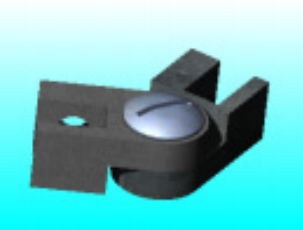
\includegraphics[height=2.5cm]{png/charniere1}

\textit{Produit désiré par l'utilisateur}
\end{center}
\end{minipage} \hfill
\begin{minipage}[c]{.3\linewidth}
\begin{center}
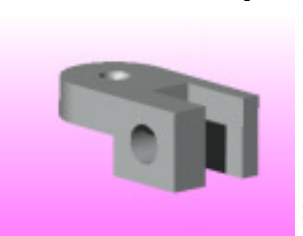
\includegraphics[height=2.5cm]{png/charniere2}

\textit{Produit issu de la conception}
\end{center}
\end{minipage} \hfill
\begin{minipage}[c]{.3\linewidth}
\begin{center}
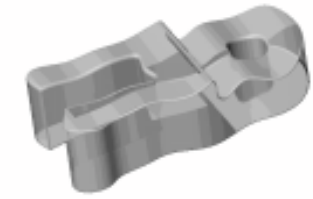
\includegraphics[height=2.5cm]{png/charniere3}

\textit{Produit issu de la fabrication}
\end{center}
\end{minipage}

\vspace{.5cm}


Beaucoup de raisons peuvent expliquer que, généralement, le produit acheté par un consommateur n'est pas exactement le même que celui qu'il aurait désiré. Outre le coût que pourrait avoir un tel produit, il est d'abord difficile pour le concepteur de créer un produit qui conviendrait à l'ensemble des utilisateurs. Ensuite, le produit réalisé en CAO à la particularité d'avoir des dimensions "parfaites". Cependant, il est impossible pour le fabriquant de réaliser des pièces "parfaites". L'ensemble des défauts des moyens de production feront que la pièce réalisée ne sera pas totalement identique au produit initialement conçu. 

A une échelle un peu plus réduite, on se demande comment deux pièces fabriquées indépendamment peuvent s'assembler à coup sûr.




%\begin{center}
%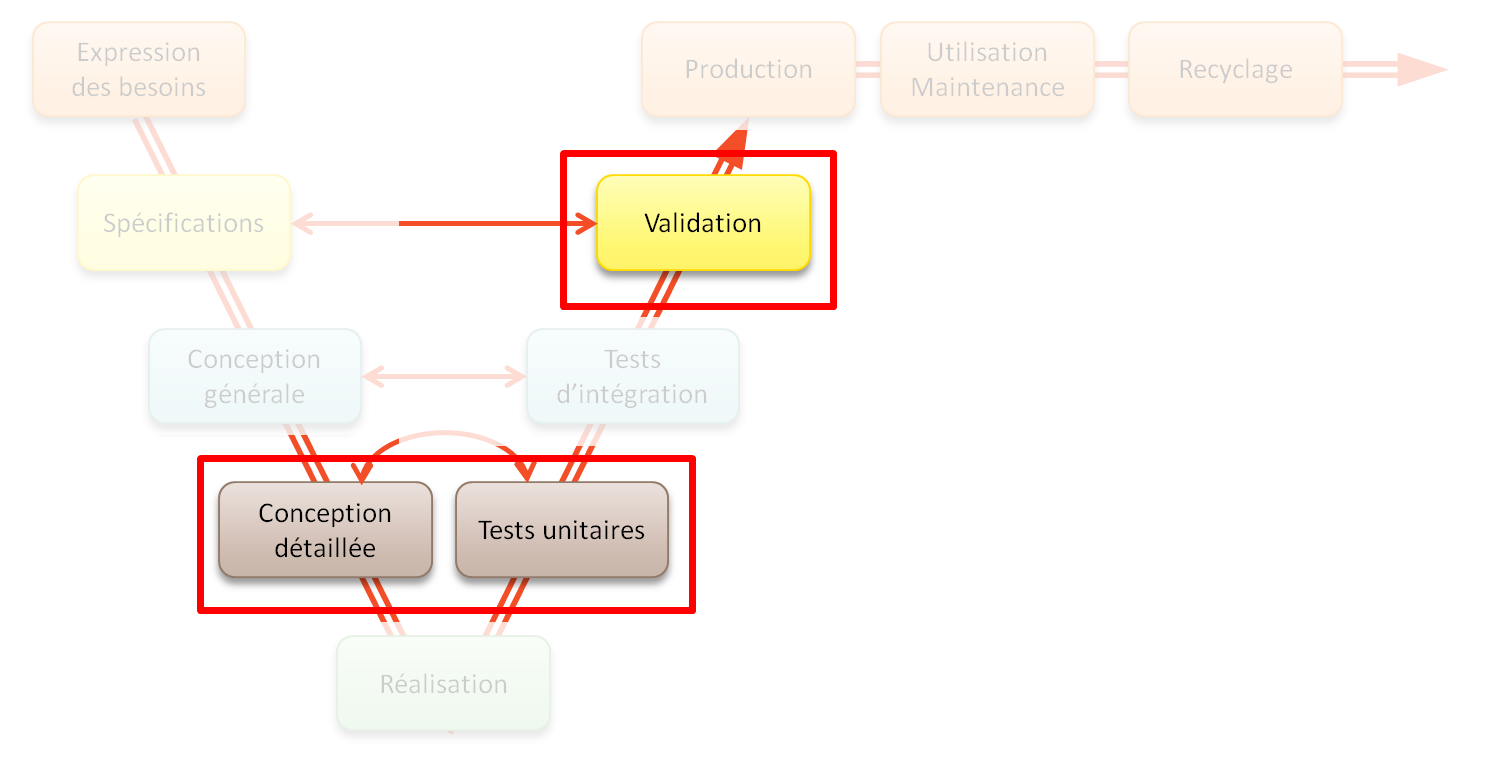
\includegraphics[width=.9\textwidth]{png/cyclev.png}

%\textit{Cycle de conception d'un produit}
%\end{center}

%\begin{prob}
%\textsc{Problématique :}

%En phase d'avant conception d'un produit, quels sont les critères qui vont permettre de choisir les matériaux à utiliser ?
%\end{prob}



\begin{savoir}
\textsc{Savoirs :}
\begin{itemize}
\item Disposer des cotes sur un dessin de façon normalisée
\item Lire et interpréter une spécification géométrique ou dimensionnelle
\end{itemize}
\end{savoir}
 

\setlength{\parskip}{0ex plus 0.2ex minus 0ex}
 \renewcommand{\contentsname}{}
 \renewcommand{\baselinestretch}{1}

\tableofcontents

 \renewcommand{\baselinestretch}{1.2}
\setlength{\parskip}{2ex plus 0.5ex minus 0.2ex}

% \vspace{1cm}
\textit{Ce document évolue. Merci de signaler toutes erreurs ou coquilles.}



\section{Quelques concepts}

Les moyens de production utilisés pour fabriquer des produits ne permettent pas de réaliser des pièces ayant des qualités dimensionnelles et géométriques parfaites. Cependant, le produit final devra quand même fonctionner avec des pièces non parfaites. 

Ainsi, une fois le produit « idéal » conçu par le concepteur, il devra alors préciser quels seront les intervalles de tolérance et les zones de tolérances sur les pièces fabriquées afin de garantir l'assemblage. 

Les difficultés de la lecture des spécifications sont les suivantes :
\begin{itemize}
\item dissocier les éléments géométriques réels (non parfaits, non idéaux) et les éléments géométriques parfaits (ou idéaux);
\item connaître le vocabulaire associé à ces éléments géométriques;
\item connaître les critères d'association entre éléments géométriques idéaux et non idéaux. 
\end{itemize}

Le but de ce cours sera donc d'interpréter les spécifications présentes sur un dessin de définition. 
\begin{minipage}[c]{.46\linewidth}
\begin{center}
\rotatebox{90}{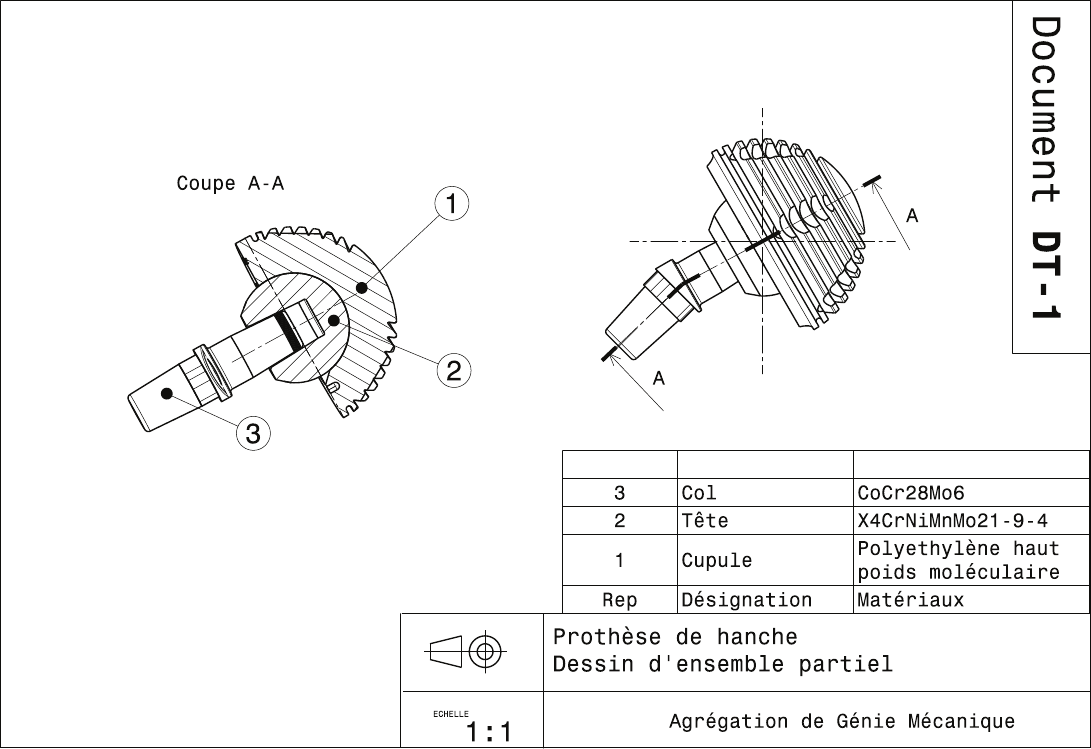
\includegraphics[height=.95\textwidth]{png/dessin_ens}}

\textit{Dessin d'ensemble}
\end{center}
\end{minipage}\hfill
\begin{minipage}[c]{.46\linewidth}
\begin{center}
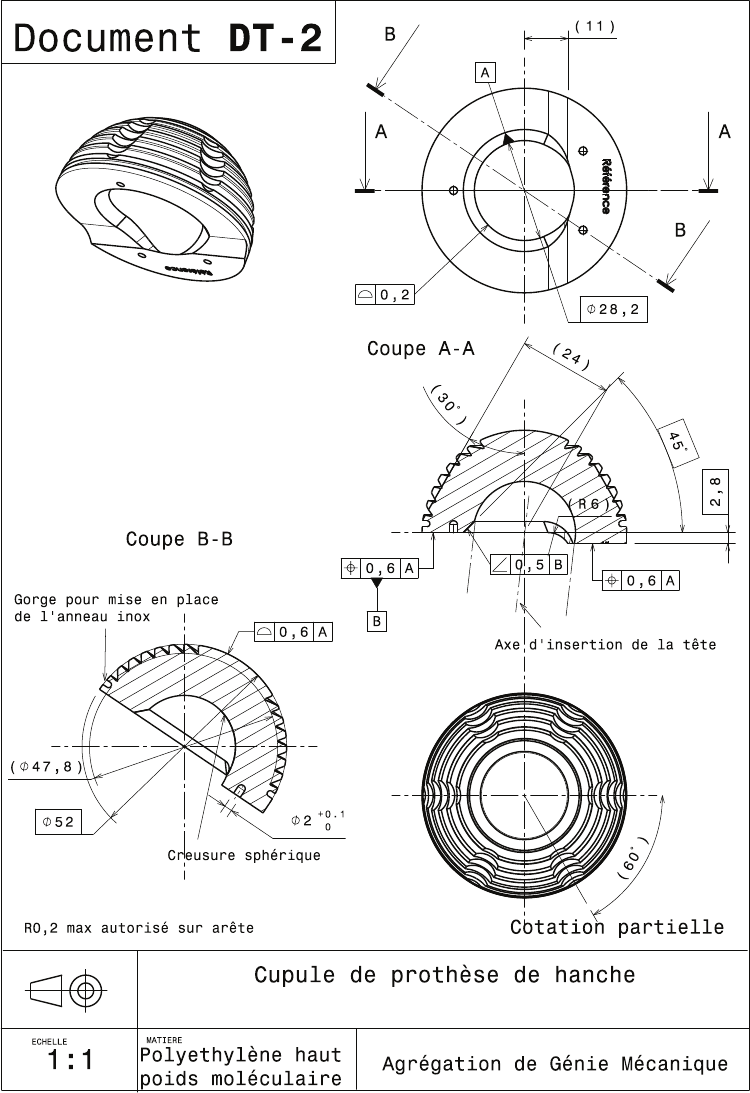
\includegraphics[width=.95\textwidth]{png/dessin_def}

\textit{Dessin de définition}
\end{center}
\end{minipage}

\begin{resultat}
\textbf{Principe de l'indépendance} \textit{[NF E 04-561], [ISO 8015]}

Chaque exigence dimensionnelle ou géométrique spécifiée sur un dessin doit être respectée en elle-même sauf indication particulière.

\end{resultat}



\section{Tolérancement dimensionnel}

\subsection{Tolérancement linéaire}

\begin{resultat}
\textbf{Tolérancement linéaire} \textit{[NF E 04-561], [ISO 8015]}

Une tolérance linéaire limite uniquement les dimensions locales réelles (\textbf{distances entre deux points}) d'un élément simple.

\end{resultat}

\begin{resultat}
\begin{minipage}[t]{.3\linewidth}
\begin{center}
Spécification

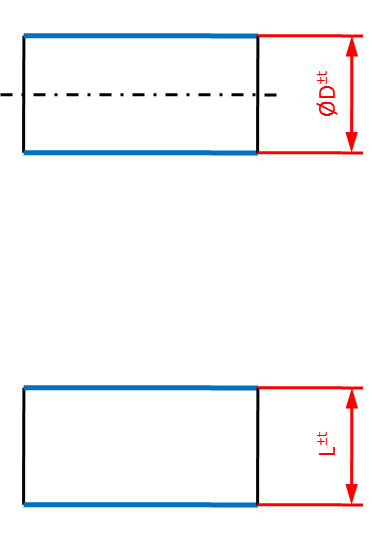
\includegraphics[width=.95\textwidth]{png/lin}
\end{center}
\end{minipage} \hfill
\begin{minipage}[t]{.3\linewidth}
\begin{center}
Interprétation
\end{center}

La pièce est dite conforme si toutes les dimensions locales $d_i$ sont comprises entre $D-t$ et $D+t$.
\end{minipage} \hfill
\begin{minipage}[t]{.3\linewidth}
\begin{center}
Interprétation géométrique

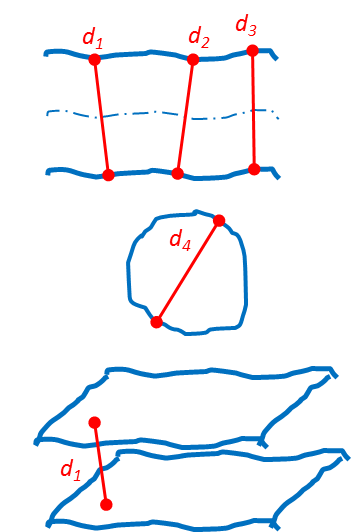
\includegraphics[width=.95\textwidth]{png/lin_int}
\end{center}
\end{minipage}
\end{resultat}




\begin{exemple}
\textit{Cylindre de révolution}

\begin{minipage}[t]{.3\linewidth}
\begin{center}
Spécification

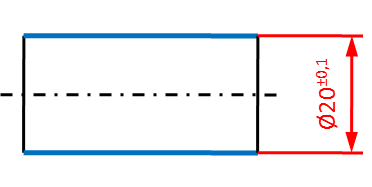
\includegraphics[width=.95\textwidth]{png/lin_cyl}
\end{center}
\end{minipage} \hfill
\begin{minipage}[t]{.3\linewidth}
\begin{center}
Interprétation
\end{center}

La pièce est dite conforme si toutes les dimensions locales réelles $d_i$ sont comprises entre $D-t$ et $D+t$.
\end{minipage} \hfill
\begin{minipage}[t]{.3\linewidth}
\begin{center}
Interprétation géométrique

\end{center}
\end{minipage}

\end{exemple}

\newpage

\begin{exemple}
\textit{Distance entre deux plans parallèles}

\begin{minipage}[t]{.3\linewidth}
\begin{center}
Spécification

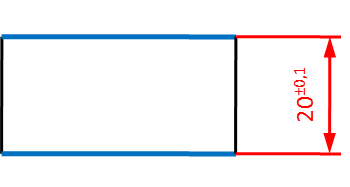
\includegraphics[width=.95\textwidth]{png/lin_plan}
\end{center}
\end{minipage} \hfill
\begin{minipage}[t]{.3\linewidth}
\begin{center}
Interprétation
\end{center}

La pièce est dite conforme si toutes les dimensions locales réelles $l_i$ sont comprises entre $L-t$ et $L+t$.
\end{minipage} \hfill
\begin{minipage}[t]{.3\linewidth}
\begin{center}
Interprétation géométrique

%\includegraphics[width=.95\textwidth]{png/}
\end{center}
\end{minipage}

\end{exemple}


\begin{warn}
La norme limite les tolérances linéaires aux cas où la distance entre deux points existe physiquement. Ainsi, on ne peut pas coter une distance entre 2 axes.
\end{warn}

\begin{exemple}
\begin{center}
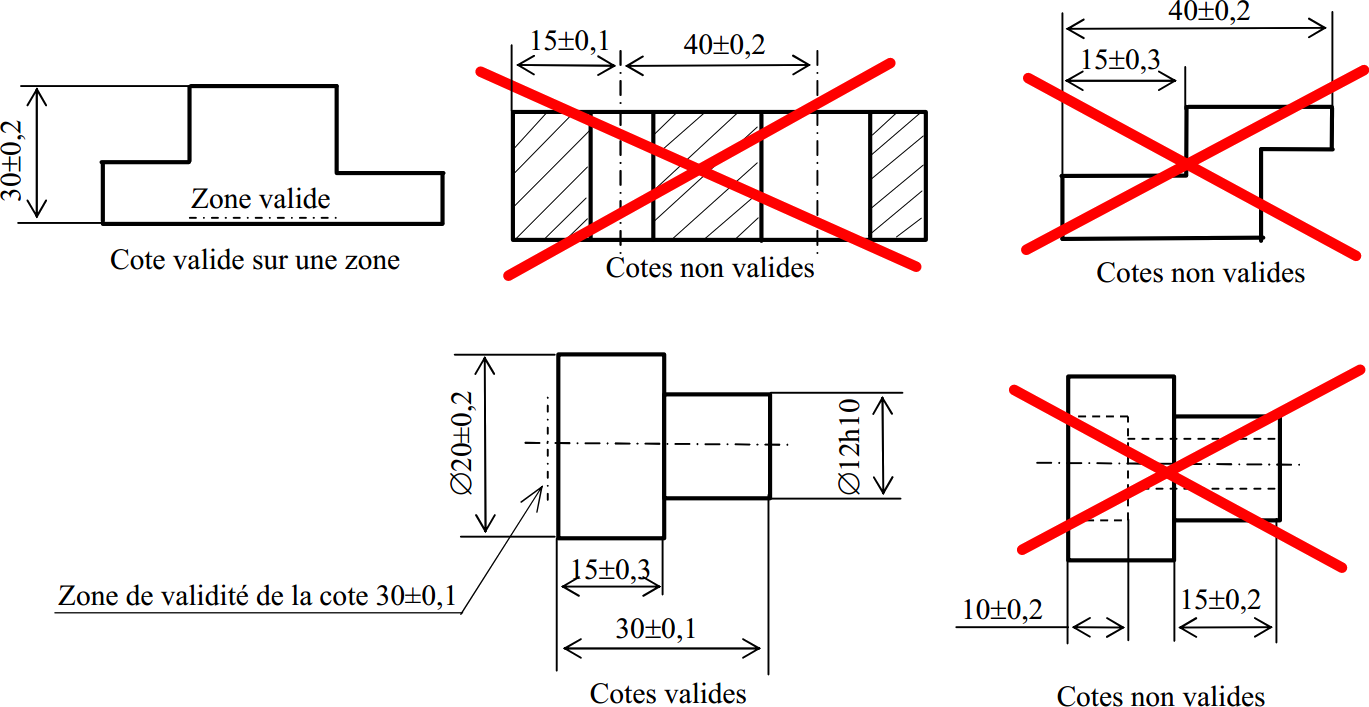
\includegraphics[width=.95\textwidth]{png/ex_nonvalide}
\end{center}
\end{exemple}

\newpage

\subsection{L'exigence de l'enveloppe}

\begin{resultat}
\textbf{L'exigence de l'enveloppe}

\begin{minipage}[t]{.3\linewidth}
\begin{center}
Spécification

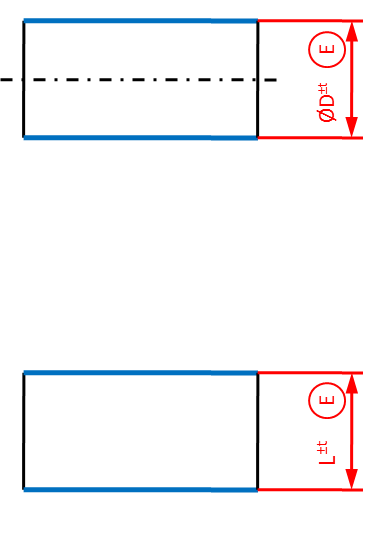
\includegraphics[width=.95\textwidth]{png/linE}
\end{center}
\end{minipage} \hfill
\begin{minipage}[t]{.3\linewidth}
\begin{center}
Interprétation
\end{center}

La pièce est dite conforme si :
\begin{itemize}
\item toutes les dimensions locales $d_i$ sont comprises entre $D-t$ et $D+t$;
\item l'enveloppe parfaite au maximum de matière n'est pas dépassée.
\end{itemize}

Cette dernière exigence peut aussi s'interpréter à l'aide d'un gabarit.
\end{minipage} \hfill
\begin{minipage}[t]{.3\linewidth}
\begin{center}
Interprétation géométrique

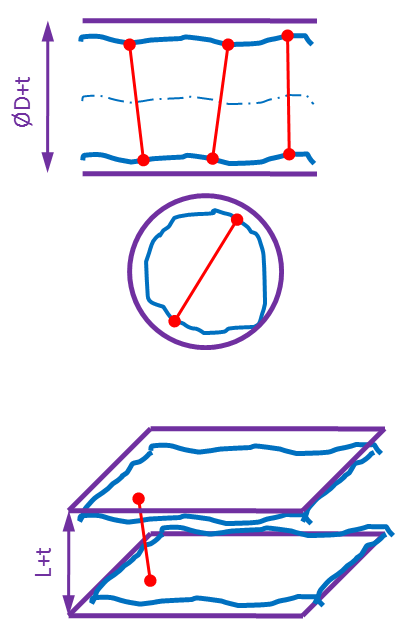
\includegraphics[width=.95\textwidth]{png/linE_int}
\end{center}
\end{minipage}
\end{resultat}

\begin{exemple}
\textit{Cylindre de révolution}

\begin{minipage}[t]{.3\linewidth}
\begin{center}
Spécification

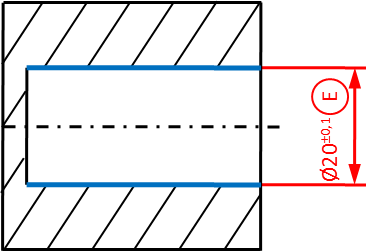
\includegraphics[width=.95\textwidth]{png/linE_cyl}
\end{center}
\end{minipage} \hfill
\begin{minipage}[t]{.3\linewidth}
\begin{center}
Interprétation
\end{center}
La pièce est dite conforme si :
\begin{itemize}
\item toutes les dimensions locales $d_i$ sont comprises entre $D-t$ et $D+t$;
\item l'enveloppe parfaite au maximum de matière n'est pas dépassée. L'enveloppe est ici un cylindre de diamètre $D+t$.
\end{itemize}

\end{minipage} \hfill
\begin{minipage}[t]{.3\linewidth}
\begin{center}
Interprétation géométrique

%\includegraphics[width=.95\textwidth]{png/}
\end{center}
\end{minipage}

\end{exemple}

\newpage

\begin{exemple}
\textit{Distance entre deux plans parallèles}

\begin{minipage}[t]{.3\linewidth}
\begin{center}
Spécification

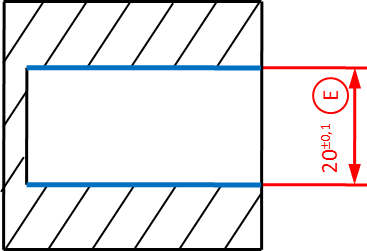
\includegraphics[width=.95\textwidth]{png/linE_plan}
\end{center}
\end{minipage} \hfill
\begin{minipage}[t]{.3\linewidth}
\begin{center}
Interprétation
\end{center}
La pièce est dite conforme si :
\begin{itemize}
\item toutes les dimensions locales $d_i$ sont comprises entre $D-t$ et $D+t$;
\item l'enveloppe parfaite au maximum de matière n'est pas dépassée. L'enveloppe est ici composée de deux plans distants de $D+t$.
\end{itemize}

\end{minipage} \hfill
\begin{minipage}[t]{.3\linewidth}
\begin{center}
Interprétation géométrique

%\includegraphics[width=.95\textwidth]{png/}
\end{center}
\end{minipage}

\end{exemple}


\subsection{Tolérancement angulaire}
\begin{resultat}
\textbf{Tolérancement angulaire} \textit{[ISO 2768-1]}

Une tolérance angulaire limite uniquement l'orientation générale \textbf{des lignes ou des éléments linéaires} des surfaces. 

\end{resultat}

\begin{exemple}
\textit{}

\begin{minipage}[t]{.3\linewidth}
\begin{center}
Spécification

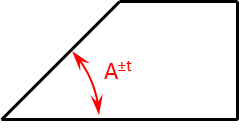
\includegraphics[width=.95\textwidth]{png/ang}
\end{center}
\end{minipage} \hfill
\begin{minipage}[t]{.3\linewidth}
\begin{center}
Interprétation
\end{center}
\end{minipage} \hfill
\begin{minipage}[t]{.3\linewidth}
\begin{center}
Interprétation géométrique

%\includegraphics[width=.95\textwidth]{png/}
\end{center}
\end{minipage}
\end{exemple}


\section{Tolérancement géométrique}

\subsection{Présentation}

L'objectif du tolérancement géométrique est multiple : lors de la phase de conception il permet de définir des spécifications géométriques qui doivent assurer que différentes pièces pourront s'assembler. Lors de la fabrication, il permet de faire en sorte que les moyens de fabrication utilisés soient compatibles avec les pièces qu'on cherche à fabriquer. Lors du contrôle des produits finis, le tolérancement géométrique doit permettre de s'assurer que la pièce fabriquée est compatible avec le cahier des charges. 

Le principe du tolérancement géométrique est de définir les variations géométriques que peut avoir la pièce. Ainsi, pour chaque surface fonctionnelle d'un produit, il permet de définir une \textbf{zone de tolérance} géométriquement \textbf{parfaite}. On devra alors vérifier, que chacune des surfaces fonctionnelles de la pièce \textbf{réelle} appartient à cette zone de tolérance. 

\begin{defi}
\begin{minipage}[c]{.4\linewidth}
Une tolérance géométrique comporte :
\begin{itemize}
\item l' (ou les) élément(s) tolérancé(s);
\item le symbole de la spécification;
\item l'étendue de la zone de tolérance;
\item \textbf{dans certains cas} une (ou un système) de référence(s) spécifiée(s). Dans ce cas, les éléments de référence sont précisés sur le dessin de définition.
\end{itemize}
\end{minipage}
\begin{minipage}[c]{.55\linewidth}
\begin{center}
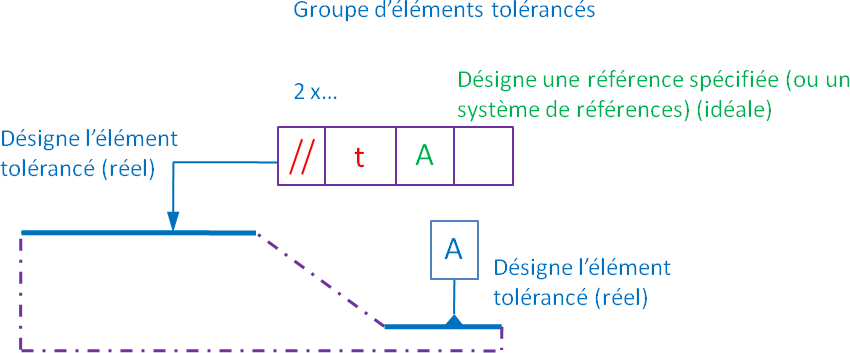
\includegraphics[width=.95\textwidth]{png/specification}
\end{center}
\end{minipage}
\end{defi}

\subsubsection{Éléments tolérancés}
\begin{defi}
Les éléments tolérancés sont des éléments réels. Ils peuvent être des points, des « lignes réelles », des « surfaces réelles ». 
Ils sont désignés par une flèche pointant une surface de la pièce.
\end{defi}

\paragraph*{Élément tolérancé unique}
\begin{exemple}

\textit{Éléments extraits de la surface réelle}

\begin{minipage}[t]{.45\linewidth}
\begin{center}
Spécification

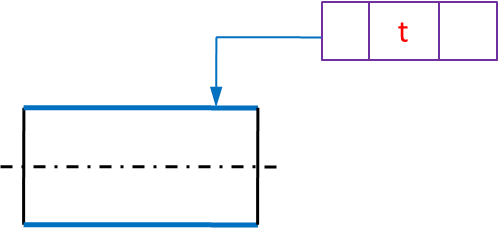
\includegraphics[width=.95\textwidth]{png/et_cyl}
\end{center}
\end{minipage} \hfill
\begin{minipage}[t]{.45\linewidth}
\begin{center}
\textbf{Élément tolérancé}
\end{center}

L'élément tolérancé est une surface \textbf{nominalement plane}.
\end{minipage} 

\begin{minipage}[t]{.45\linewidth}
\begin{center}
Spécification

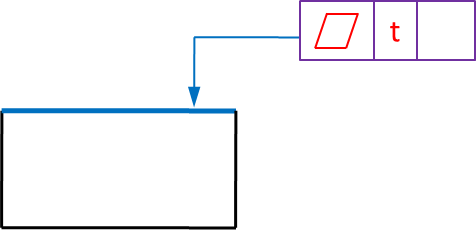
\includegraphics[width=.95\textwidth]{png/et_plan}
\end{center}
\end{minipage} \hfill
\begin{minipage}[t]{.45\linewidth}
\begin{center}
\textbf{Élément tolérancé}
\end{center}

L'élément tolérancé est une surface \textbf{nominalement cylindrique}.
\end{minipage} 
\end{exemple}

\begin{exemple}

\textit{Éléments tolérancés construits}

\begin{minipage}[t]{.45\linewidth}
\begin{center}
Spécification

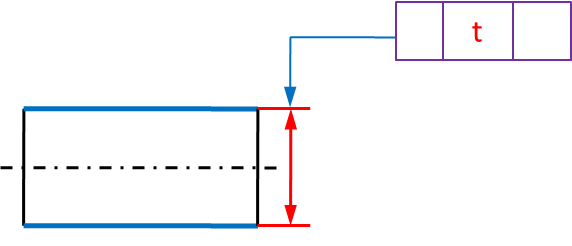
\includegraphics[width=.95\textwidth]{png/et_cycl_cons}
\end{center}
\end{minipage} \hfill
\begin{minipage}[t]{.45\linewidth}
\begin{center}
\textbf{Élément tolérancé}
\end{center}

L'élément tolérancé est \textbf{l'axe réel d'une surface nominalement cylindrique}.
\end{minipage} 

\begin{minipage}[t]{.45\linewidth}
\begin{center}
Spécification

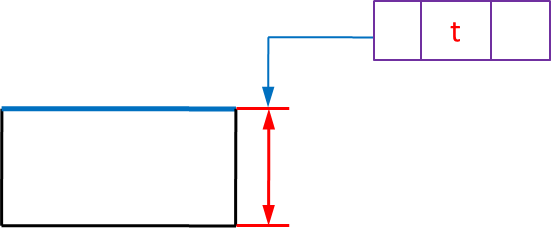
\includegraphics[width=.95\textwidth]{png/et_plan_cons}
\end{center}
\end{minipage} \hfill
\begin{minipage}[t]{.45\linewidth}
\begin{center}
\textbf{Élément tolérancé}
\end{center}

L'élément tolérancé est une surface \textbf{médiane nominalement plane}.
\end{minipage} 
\end{exemple}

\begin{rem}
Les éléments tolérancés sont construits lorsque la flèche désignant l'élément tolérancé est situé en face d'une ligne de cote bilimite. 
\end{rem}


\begin{rem}
\textit{Construction d'un élément tolérancé construit}
\end{rem}
\paragraph*{Groupe d'éléments tolérancés}


\begin{exemple}

On parle de groupe d'éléments tolérancés lorsqu'on précise un nombre au dessus de la spécification géométrique.

\begin{minipage}[t]{.45\linewidth}
\begin{center}
Spécification

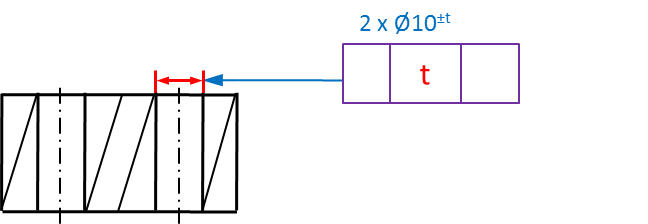
\includegraphics[width=.95\textwidth]{png/et_gr}
\end{center}
\end{minipage} \hfill
\begin{minipage}[t]{.45\linewidth}
\begin{center}
\textbf{Éléments tolérancés}
\end{center}


\end{minipage} 
\end{exemple}


\subsubsection{Éléments de référence et référence spécifiée}
\begin{defi}

\textbf{Élément de référence}

L'élément de référence est un élément réel issu du skin modèle. Cette élément est désigné par un triangle noirci.
\end{defi}

\begin{defi}
\textbf{Référence spécifiée}

La référence spécifiée est un élément idéal. Ce ne peut être qu'un \textbf{point}, une \textbf{droite} ou un \textbf{plan}.

La référence spécifiée est \textbf{construite géométriquement} à partir de l'élément de référence. 
\end{defi}

\begin{rem}
\textbf{Critères d'association} -- la RS est toujours extérieure à la matière.

\begin{center}
\begin{tabular}{p{.45\textwidth} p{.45\textwidth}}
L'élément de référence est : & La référence spécifiée peut être :\\
Une surface nominalement plane & Le plan tangent extérieur matière qui  minimise le défaut de forme \\
Une surface nominalement cylindrique & 
\begin{itemize}
\item L'axe du plus grand cylindre inscrit qui minimise le défaut de forme
\item L'axe du plus petit cylindre circonscrit qui minimise le défaut de forme
\end{itemize}
\\
Une ligne nominalement circulaire & 
\begin{itemize}
\item Le point centre du plus grand cercle inscrit
\item Le point centre du plus petit cercle circonscrit
\end{itemize}
\\
\end{tabular}
\end{center}

\end{rem}

\begin{exemple}
\begin{minipage}[t]{.3\linewidth}
$\;$

\begin{center}
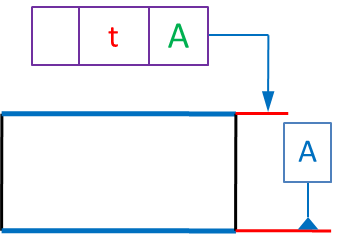
\includegraphics[width=.95\textwidth]{png/rs_plan}
\end{center}
\end{minipage} \hfill
\begin{minipage}[t]{.3\linewidth}
\textbf{ER} : Surface nominalement plane

\textbf{RS} : Plan tangent extérieur matière qui minimise le défaut de forme
\end{minipage} \hfill
\begin{minipage}[t]{.3\linewidth}
\begin{center}
%\includegraphics[width=.95\textwidth]{png/}
\end{center}
\end{minipage} 
\end{exemple}


\begin{exemple}
\begin{minipage}[t]{.3\linewidth}
\begin{center}
$\;$

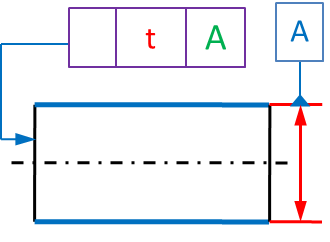
\includegraphics[width=.95\textwidth]{png/rs_cyl}
\end{center}
\end{minipage} \hfill
\begin{minipage}[t]{.3\linewidth}
\textbf{ER} : Surface nominalement cylindrique

\textbf{RS} : \textbf{AXE} du plus grand cylindre inscrit qui minimise le défaut de forme.
\end{minipage} \hfill
\begin{minipage}[t]{.3\linewidth}
\begin{center}
%\includegraphics[width=.95\textwidth]{png/}
\end{center}
\end{minipage} 
\end{exemple}



\subsubsection{Systèmes de références spécifiées}

\begin{defi}
Lorsque plusieurs références spécifiées sont précisées dans le cadre de la tolérance, on parle de systèmes de références spécifiées. 

La première référence spécifiée est construite avec un critère d'association usuel par rapport à l'élément de référence primaire. La référence secondaire doit être contrainte par rapport à la référence primaire (contrainte d'orthogonalité ou de parallélisme). Il en est de même pour la référence spécifiée secondaire. 
\end{defi}



\begin{exemple}
\begin{minipage}[t]{.3\linewidth}
\begin{center}
$\;$

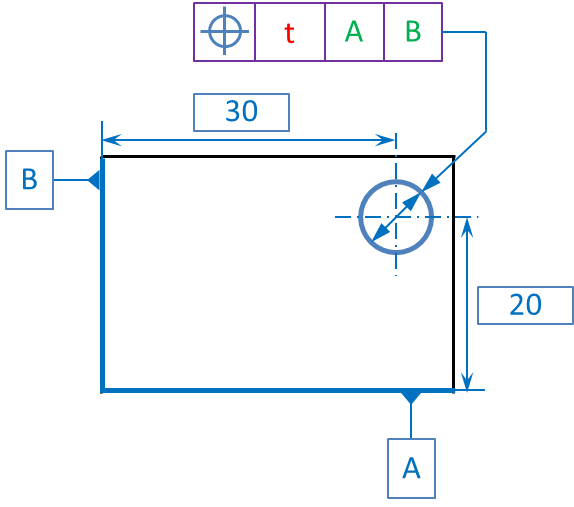
\includegraphics[width=.95\textwidth]{png/rs_syst}
\end{center}
\end{minipage} \hfill
\begin{minipage}[t]{.3\linewidth}
\textbf{ER} : 
\begin{itemize}
\item élément de référence primaire : surface nominalement plane
\item élément de référence secondaire : surface nominalement plane
\end{itemize}
\textbf{RS} :
\begin{itemize}
\item référence spécifiée primaire : plan tangent extérieur matière qui minimise le défaut de forme
\item référence spécifiée secondaire : plan tangent extérieur matière qui minimise le défaut de forme et qui est perpendiculaire à la RS primaire.
\end{itemize} 
\end{minipage} \hfill
\begin{minipage}[t]{.3\linewidth}
\begin{center}
%\includegraphics[width=.95\textwidth]{png/}
\end{center}
\end{minipage} 
\end{exemple}

\begin{exemple}
\begin{minipage}[t]{.3\linewidth}
\begin{center}
$\;$

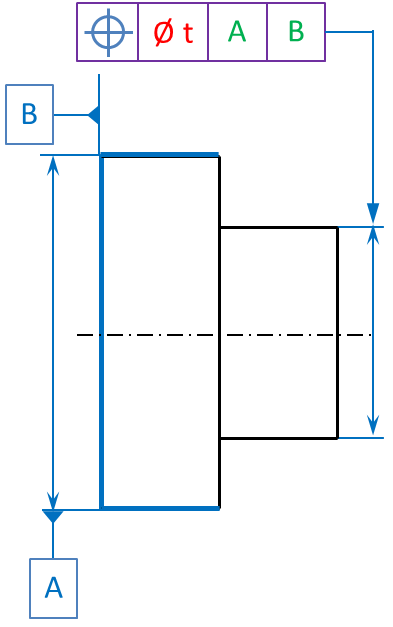
\includegraphics[width=.95\textwidth]{png/rs_syst2}
\end{center}
\end{minipage} \hfill
\begin{minipage}[t]{.3\linewidth}
\textbf{ER} : 
\begin{itemize}
\item élément de référence primaire : surface nominalement plane;
\item élément de référence secondaire : surface nominalement cylindrique.
\end{itemize}
\textbf{RS} :
\begin{itemize}
\item référence spécifiée primaire : plan tangent extérieur matière qui minimise le défaut de forme;
\item référence spécifiée secondaire : axe du plus grand cylindre inscrit qui minimise le défaut de forme et qui est perpendiculaire à la RS primaire.
\end{itemize} 
\end{minipage} \hfill
\begin{minipage}[t]{.3\linewidth}
\begin{center}
%\includegraphics[width=.95\textwidth]{png/}
\end{center}
\end{minipage} 
\end{exemple}


\subsubsection{Zones communes}

\begin{exemple}
\begin{minipage}[t]{.3\linewidth}
\begin{center}
$\;$

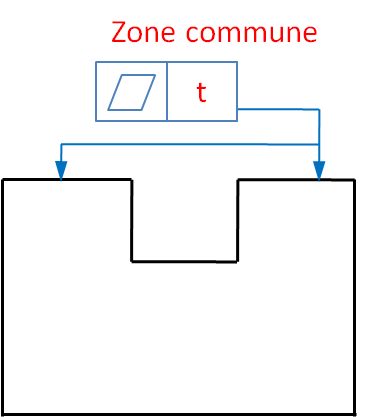
\includegraphics[width=.95\textwidth]{png/ex_zc}
\end{center}
\end{minipage} \hfill
\begin{minipage}[t]{.6\linewidth}

\end{minipage}
\end{exemple}

\subsubsection{Zones de tolérance}
\begin{defi}
\textbf{Zone de tolérance}

Une zone de tolérance est un volume ou une surface géométrique parfait. Afin de garantir la conformité de la pièce, il est nécessaire que l'élément tolérance soit situé dans la zone de tolérance.

La zone de tolérance est \textbf{unique} si l'élément tolérancé est unique. La zone de tolérance est composée lorsqu'on prend en compte un groupe d'éléments tolérancés. 

La forme de la zone de tolérance dépend du symbole de la spécificationde la nature de l'élément tolérancé et du modificateur se situant devant la valeur de la tolérance. 
\end{defi}

\begin{resultat}
\begin{center}
\begin{tabular}{cl}
\multicolumn{2}{c}{\textbf{Spécifications de forme}} \\

\includegraphics[width=.5cm]{png/rectitude}
& Rectitude \\

\includegraphics[width=.5cm]{png/circularite}
& Circularité\\

\includegraphics[width=.5cm]{png/planeite}
& Planéité \\

\includegraphics[width=.5cm]{png/cylindricite}
& Cylindricité \\

\includegraphics[width=.5cm]{png/ligne}
& Forme d'une ligne quelconque\\

\includegraphics[width=.5cm]{png/surface}
& Forme d'une surface quelconque\\
\end{tabular}
\begin{tabular}{cl}
\multicolumn{2}{c}{\textbf{Spécifications d'orientation}} \\

\includegraphics[width=.5cm]{png/parallelisme}
& Parallélisme \\
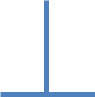
\includegraphics[width=.5cm]{png/perpendicularite}
& Perpendicularité \\

\includegraphics[width=.5cm]{png/inclinaison}
& Inclinaison \\

\includegraphics[width=.5cm]{png/ligne}
& Orientation d'une ligne quelconque\\

\includegraphics[width=.5cm]{png/surface}
& Orientation d'une surface quelconque\\
\end{tabular}
\end{center}

\begin{center}
\begin{tabular}{cl}
\multicolumn{2}{c}{\textbf{Spécifications de position}}\\

\includegraphics[width=.5cm]{png/symetrie}
& Symétrie\\

\includegraphics[width=.5cm]{png/coaxialite}
& Concentricité\\

\includegraphics[width=.5cm]{png/coaxialite}
& Coaxialité \\
\includegraphics[width=.5cm]{png/localisation}
& Localisation \\
\includegraphics[width=.5cm]{png/ligne}
& Position d'une ligne quelconque\\
\includegraphics[width=.5cm]{png/surface}
& Position d'une surface quelconque\\
\end{tabular}
\begin{tabular}{cl}
\multicolumn{2}{c}{\textbf{Spécifications de battement}}\\
\includegraphics[width=.5cm]{png/battements}
& Battement circulaire \\
\includegraphics[width=.5cm]{png/battementt}
& Battement total\\
\end{tabular}
\end{center}

\end{resultat}




\begin{exemple}
\begin{minipage}[t]{.3\linewidth}
\begin{center}
$\;$ 

\includegraphics[width=.95\textwidth]{png/zt_plan}
\end{center}
\end{minipage} \hfill
\begin{minipage}[t]{.3\linewidth}
\textbf{Zone de tolérance :}

Zone comprise entre deux plans parallèles distants de $t$.
\end{minipage} \hfill
\begin{minipage}[t]{.3\linewidth}
\begin{center}
%\includegraphics[width=.95\textwidth]{png/}
\end{center}
\end{minipage} 
\end{exemple}


\begin{exemple}
\begin{minipage}[t]{.3\linewidth}
\begin{center}
$\;$ 

\includegraphics[width=.95\textwidth]{png/zt_cyl}
\end{center}
\end{minipage} \hfill
\begin{minipage}[t]{.3\linewidth}
\textbf{Zone de tolérance :}

Cylindre de diamètre $t$.
\end{minipage} \hfill
\begin{minipage}[t]{.3\linewidth}
\begin{center}
%\includegraphics[width=.95\textwidth]{png/}
\end{center}
\end{minipage} 
\end{exemple}

%\begin{exemple}
%\begin{minipage}[t]{.3\linewidth}
%\begin{center}
%%\includegraphics[width=.95\textwidth]{png/}
%\end{center}
%\end{minipage} \hfill
%\begin{minipage}[t]{.3\linewidth}
%\textbf{Zone de tolérance :}
%
%Zone comprise entre 2 cylindres coaxiaux distants de $t$. 
%\end{minipage} \hfill
%\begin{minipage}[t]{.3\linewidth}
%\begin{center}
%%\includegraphics[width=.95\textwidth]{png/}
%\end{center}
%\end{minipage} 
%\end{exemple}


\begin{exemple}
\begin{minipage}[t]{.3\linewidth}
\begin{center}
$\;$

\includegraphics[width=.95\textwidth]{png/zt_1}
\end{center}
\end{minipage} \hfill
\begin{minipage}[t]{.3\linewidth}
\textbf{Zone de tolérance :}

\end{minipage} \hfill
\begin{minipage}[t]{.3\linewidth}
\begin{center}
%\includegraphics[width=.95\textwidth]{png/}
\end{center}
\end{minipage} 
\end{exemple}

\begin{exemple}
\begin{minipage}[t]{.3\linewidth}
\begin{center}
$\;$

\includegraphics[width=.95\textwidth]{png/zt_2}
\end{center}
\end{minipage} \hfill
\begin{minipage}[t]{.3\linewidth}
\textbf{Zone de tolérance :}

\end{minipage} \hfill
\begin{minipage}[t]{.3\linewidth}
\begin{center}
%\includegraphics[width=.95\textwidth]{png/}
\end{center}
\end{minipage} 
\end{exemple}

\newpage

\subsection{Spécifications de forme}

\begin{exemple}
\footnotesize{
\begin{center}
\begin{tabular}{|p{.14\textwidth}|p{.14\textwidth}|p{.14\textwidth}|p{.14\textwidth}|p{.14\textwidth}|p{.14\textwidth}|}
\hline
Symbole de la spécification & 
\multicolumn{2}{c|}{Éléments non idéaux} &
\multicolumn{3}{c|}{Élément idéaux} \\
&
\multicolumn{2}{c|}{} &
\multicolumn{3}{c|}{}\\
\hline
Type de spécification & 
Éléments tolérancés &
Éléments de référence & 
Référence spécifiée & 
\multicolumn{2}{c|}{Zone de tolérance} \\
&&&&
\multicolumn{2}{c|}{}\\
\hline
Condition de conformité & 
Unique Groupe & Unique Multiples &
Simple Commune Système &
Simple Composée & 
Contraintes et/ou position \\
\hline
\multirow{12}{*}{\includegraphics[width=2cm]{png/ex_rectitude}}&&&&&\\
&&&&&\\
&&&&&\\
&&&&&\\
&&&&&\\
&&&&&\\
&&&&&\\
&&&&&\\
&&&&&\\
&&&&&\\
&&&&&\\
&&&&&\\
\hline
\end{tabular}
\end{center}
}
\end{exemple}

\begin{exemple}
\footnotesize{
\begin{center}
\begin{tabular}{|p{.14\textwidth}|p{.14\textwidth}|p{.14\textwidth}|p{.14\textwidth}|p{.14\textwidth}|p{.14\textwidth}|}
\hline
Symbole de la spécification & 
\multicolumn{2}{c|}{Éléments non idéaux} &
\multicolumn{3}{c|}{Élément idéaux} \\
&
\multicolumn{2}{c|}{} &
\multicolumn{3}{c|}{}\\
\hline
Type de spécification & 
Éléments tolérancés &
Éléments de référence & 
Référence spécifiée & 
\multicolumn{2}{c|}{Zone de tolérance} \\
&&&&
\multicolumn{2}{c|}{}\\
\hline
Condition de conformité & 
Unique Groupe & Unique Multiples &
Simple Commune Système &
Simple Composée & 
Contraintes et/ou position \\
\hline
\multirow{12}{*}{\includegraphics[width=2cm]{png/ex_circularite}}&&&&&\\
&&&&&\\
&&&&&\\
&&&&&\\
&&&&&\\
&&&&&\\
&&&&&\\
&&&&&\\
&&&&&\\
&&&&&\\
&&&&&\\
&&&&&\\
\hline
\end{tabular}
\end{center}
}
\end{exemple}

\begin{exemple}
\footnotesize{
\begin{center}
\begin{tabular}{|p{.14\textwidth}|p{.14\textwidth}|p{.14\textwidth}|p{.14\textwidth}|p{.14\textwidth}|p{.14\textwidth}|}
\hline
Symbole de la spécification & 
\multicolumn{2}{c|}{Éléments non idéaux} &
\multicolumn{3}{c|}{Élément idéaux} \\
&
\multicolumn{2}{c|}{} &
\multicolumn{3}{c|}{}\\
\hline
Type de spécification & 
Éléments tolérancés &
Éléments de référence & 
Référence spécifiée & 
\multicolumn{2}{c|}{Zone de tolérance} \\
&&&&
\multicolumn{2}{c|}{}\\
\hline
Condition de conformité & 
Unique Groupe & Unique Multiples &
Simple Commune Système &
Simple Composée & 
Contraintes et/ou position \\
\hline
\multirow{12}{*}{\includegraphics[width=2cm]{png/ex_planeite}}&&&&&\\
&&&&&\\
&&&&&\\
&&&&&\\
&&&&&\\
&&&&&\\
&&&&&\\
&&&&&\\
&&&&&\\
&&&&&\\
&&&&&\\
&&&&&\\
\hline
\end{tabular}
\end{center}
}
\end{exemple}

\begin{exemple}
\footnotesize{
\begin{center}
\begin{tabular}{|p{.14\textwidth}|p{.14\textwidth}|p{.14\textwidth}|p{.14\textwidth}|p{.14\textwidth}|p{.14\textwidth}|}
\hline
Symbole de la spécification & 
\multicolumn{2}{c|}{Éléments non idéaux} &
\multicolumn{3}{c|}{Élément idéaux} \\
&
\multicolumn{2}{c|}{} &
\multicolumn{3}{c|}{}\\
\hline
Type de spécification & 
Éléments tolérancés &
Éléments de référence & 
Référence spécifiée & 
\multicolumn{2}{c|}{Zone de tolérance} \\
&&&&
\multicolumn{2}{c|}{}\\
\hline
Condition de conformité & 
Unique Groupe & Unique Multiples &
Simple Commune Système &
Simple Composée & 
Contraintes et/ou position \\
\hline
\multirow{12}{*}{\includegraphics[width=2cm]{png/ex_cylindricite}}&&&&&\\
&&&&&\\
&&&&&\\
&&&&&\\
&&&&&\\
&&&&&\\
&&&&&\\
&&&&&\\
&&&&&\\
&&&&&\\
&&&&&\\
&&&&&\\
\hline
\end{tabular}
\end{center}
}
\end{exemple}



\subsection{Spécifications d'orientation}



\begin{exemple}
\footnotesize{
\begin{center}
\begin{tabular}{|p{.14\textwidth}|p{.14\textwidth}|p{.14\textwidth}|p{.14\textwidth}|p{.14\textwidth}|p{.14\textwidth}|}
\hline
Symbole de la spécification & 
\multicolumn{2}{c|}{Éléments non idéaux} &
\multicolumn{3}{c|}{Élément idéaux} \\
&
\multicolumn{2}{c|}{} &
\multicolumn{3}{c|}{}\\
\hline
Type de spécification & 
Éléments tolérancés &
Éléments de référence & 
Référence spécifiée & 
\multicolumn{2}{c|}{Zone de tolérance} \\
&&&&
\multicolumn{2}{c|}{}\\
\hline
Condition de conformité & 
Unique Groupe & Unique Multiples &
Simple Commune Système &
Simple Composée & 
Contraintes et/ou position \\
\hline
\multirow{12}{*}{\includegraphics[width=2cm]{png/ex_parallelisme}}&&&&&\\
&&&&&\\
&&&&&\\
&&&&&\\
&&&&&\\
&&&&&\\
&&&&&\\
&&&&&\\
&&&&&\\
&&&&&\\
&&&&&\\
&&&&&\\
\hline
\end{tabular}
\end{center}
}
\end{exemple}


\begin{exemple}
\footnotesize{
\begin{center}
\begin{tabular}{|p{.14\textwidth}|p{.14\textwidth}|p{.14\textwidth}|p{.14\textwidth}|p{.14\textwidth}|p{.14\textwidth}|}
\hline
Symbole de la spécification & 
\multicolumn{2}{c|}{Éléments non idéaux} &
\multicolumn{3}{c|}{Élément idéaux} \\
&
\multicolumn{2}{c|}{} &
\multicolumn{3}{c|}{}\\
\hline
Type de spécification & 
Éléments tolérancés &
Éléments de référence & 
Référence spécifiée & 
\multicolumn{2}{c|}{Zone de tolérance} \\
&&&&
\multicolumn{2}{c|}{}\\
\hline
Condition de conformité & 
Unique Groupe & Unique Multiples &
Simple Commune Système &
Simple Composée & 
Contraintes et/ou position \\
\hline
\multirow{12}{*}{\includegraphics[width=2cm]{png/ex_perpendicularite}}&&&&&\\
&&&&&\\
&&&&&\\
&&&&&\\
&&&&&\\
&&&&&\\
&&&&&\\
&&&&&\\
&&&&&\\
&&&&&\\
&&&&&\\
&&&&&\\
\hline
\end{tabular}
\end{center}
}
\end{exemple}






\subsection{Spécifications de position}

\begin{exemple}
\footnotesize{
\begin{center}
\begin{tabular}{|p{.14\textwidth}|p{.14\textwidth}|p{.14\textwidth}|p{.14\textwidth}|p{.14\textwidth}|p{.14\textwidth}|}
\hline
Symbole de la spécification & 
\multicolumn{2}{c|}{Éléments non idéaux} &
\multicolumn{3}{c|}{Élément idéaux} \\
&
\multicolumn{2}{c|}{} &
\multicolumn{3}{c|}{}\\
\hline
Type de spécification & 
Éléments tolérancés &
Éléments de référence & 
Référence spécifiée & 
\multicolumn{2}{c|}{Zone de tolérance} \\
&&&&
\multicolumn{2}{c|}{}\\
\hline
Condition de conformité & 
Unique Groupe & Unique Multiples &
Simple Commune Système &
Simple Composée & 
Contraintes et/ou position \\
\hline
\multirow{12}{*}{\includegraphics[width=2cm]{png/ex_symetrie}}&&&&&\\
&&&&&\\
&&&&&\\
&&&&&\\
&&&&&\\
&&&&&\\
&&&&&\\
&&&&&\\
&&&&&\\
&&&&&\\
&&&&&\\
&&&&&\\
\hline
\end{tabular}
\end{center}
}
\end{exemple}

\begin{exemple}
\footnotesize{
\begin{center}
\begin{tabular}{|p{.14\textwidth}|p{.14\textwidth}|p{.14\textwidth}|p{.14\textwidth}|p{.14\textwidth}|p{.14\textwidth}|}
\hline
Symbole de la spécification & 
\multicolumn{2}{c|}{Éléments non idéaux} &
\multicolumn{3}{c|}{Élément idéaux} \\
&
\multicolumn{2}{c|}{} &
\multicolumn{3}{c|}{}\\
\hline
Type de spécification & 
Éléments tolérancés &
Éléments de référence & 
Référence spécifiée & 
\multicolumn{2}{c|}{Zone de tolérance} \\
&&&&
\multicolumn{2}{c|}{}\\
\hline
Condition de conformité & 
Unique Groupe & Unique Multiples &
Simple Commune Système &
Simple Composée & 
Contraintes et/ou position \\
\hline
\multirow{12}{*}{\includegraphics[width=2cm]{png/ex_coax}}&&&&&\\
&&&&&\\
&&&&&\\
&&&&&\\
&&&&&\\
&&&&&\\
&&&&&\\
&&&&&\\
&&&&&\\
&&&&&\\
&&&&&\\
&&&&&\\
\hline
\end{tabular}
\end{center}
}
\end{exemple}

\begin{exemple}
\footnotesize{
\begin{center}
\begin{tabular}{|p{.14\textwidth}|p{.14\textwidth}|p{.14\textwidth}|p{.14\textwidth}|p{.14\textwidth}|p{.14\textwidth}|}
\hline
Symbole de la spécification & 
\multicolumn{2}{c|}{Éléments non idéaux} &
\multicolumn{3}{c|}{Élément idéaux} \\
&
\multicolumn{2}{c|}{} &
\multicolumn{3}{c|}{}\\
\hline
Type de spécification & 
Éléments tolérancés &
Éléments de référence & 
Référence spécifiée & 
\multicolumn{2}{c|}{Zone de tolérance} \\
&&&&
\multicolumn{2}{c|}{}\\
\hline
Condition de conformité & 
Unique Groupe & Unique Multiples &
Simple Commune Système &
Simple Composée & 
Contraintes et/ou position \\
\hline
\multirow{12}{*}{\includegraphics[width=2cm]{png/ex_loca}}&&&&&\\
&&&&&\\
&&&&&\\
&&&&&\\
&&&&&\\
&&&&&\\
&&&&&\\
&&&&&\\
&&&&&\\
&&&&&\\
&&&&&\\
&&&&&\\
\hline
\end{tabular}
\end{center}
}
\end{exemple}



\subsection{Spécifications  de battement}


\begin{exemple}
\footnotesize{
\begin{center}
\begin{tabular}{|p{.14\textwidth}|p{.14\textwidth}|p{.14\textwidth}|p{.14\textwidth}|p{.14\textwidth}|p{.14\textwidth}|}
\hline
Symbole de la spécification & 
\multicolumn{2}{c|}{Éléments non idéaux} &
\multicolumn{3}{c|}{Élément idéaux} \\
&
\multicolumn{2}{c|}{} &
\multicolumn{3}{c|}{}\\
\hline
Type de spécification & 
Éléments tolérancés &
Éléments de référence & 
Référence spécifiée & 
\multicolumn{2}{c|}{Zone de tolérance} \\
&&&&
\multicolumn{2}{c|}{}\\
\hline
Condition de conformité & 
Unique Groupe & Unique Multiples &
Simple Commune Système &
Simple Composée & 
Contraintes et/ou position \\
\hline
\multirow{12}{*}{\includegraphics[width=2cm]{png/ex_battements}}&&&&&\\
&&&&&\\
&&&&&\\
&&&&&\\
&&&&&\\
&&&&&\\
&&&&&\\
&&&&&\\
&&&&&\\
&&&&&\\
&&&&&\\
&&&&&\\
\hline
\end{tabular}
\end{center}
}
\end{exemple}


\begin{exemple}
\footnotesize{
\begin{center}
\begin{tabular}{|p{.14\textwidth}|p{.14\textwidth}|p{.14\textwidth}|p{.14\textwidth}|p{.14\textwidth}|p{.14\textwidth}|}
\hline
Symbole de la spécification & 
\multicolumn{2}{c|}{Éléments non idéaux} &
\multicolumn{3}{c|}{Élément idéaux} \\
&
\multicolumn{2}{c|}{} &
\multicolumn{3}{c|}{}\\
\hline
Type de spécification & 
Éléments tolérancés &
Éléments de référence & 
Référence spécifiée & 
\multicolumn{2}{c|}{Zone de tolérance} \\
&&&&
\multicolumn{2}{c|}{}\\
\hline
Condition de conformité & 
Unique Groupe & Unique Multiples &
Simple Commune Système &
Simple Composée & 
Contraintes et/ou position \\
\hline
\multirow{12}{*}{\includegraphics[width=2cm]{png/ex_battementt}}&&&&&\\
&&&&&\\
&&&&&\\
&&&&&\\
&&&&&\\
&&&&&\\
&&&&&\\
&&&&&\\
&&&&&\\
&&&&&\\
&&&&&\\
&&&&&\\
\hline
\end{tabular}
\end{center}
}
\end{exemple}

%\subsection{Exigences particulières}

%\section{États de surface}

%\section{Métrologie}

%\section{Démarche de cotation fonctionnelle}

%\section{Ajustements}

%\section{Chaînes de cotes}


\begin{thebibliography}{2}
\bibitem{gps}{\textit{Centre d'Études et de Rénovation Pédagogique de l'Enseignement Technique}, Exploitation du concept G.P.S. et de la normalisation pour la Spécification Géométrique des Produits.}
\bibitem{gps2}{\textit{Le Décodage du Dessin de Définition}, Guy Percebois, Lycée Louis Vincent -- Metz . \url{http://www.ac-nancy-metz.fr/enseign/sti/genimeca/zip/GPS/Tol\%20g\%E9o\%20pr\%E9\%20bac.pdf}}
%\bibitem{rb}{Supports de cours de Renan Bonnard,PTSI, Lycée Newton, Clichy la Garenne}
%\bibitem{jb}{Supports de cours de Joël Boiron, PTSI, Lycée Gustave Eiffel, Bordeaux}
%\bibitem{mc}{Supports de cours de Maryline Carrez, Lycée Jules Haag, Besançon}
%\bibitem{pf}{Supports de cours de Philippe Fichou, Lycée Vauban, Brest \url{http://philippe.fichou.pagesperso-orange.fr/documents/liaisoncomplete2003.pdf}}
%\bibitem{jpp}{Supports de cours de Jean-Pierre Pupier, Lycée Rouvière, Toulon}


\end{thebibliography}

\end{document}